\section{The Segment Routing (SR) architecture}
\label{sec:arch}

This section includes a short tutorial on the main SR architectural aspects. Our goal is to provide a common ground and a reference conceptual framework for the survey. RFC 8402 \cite{rfc8402} represents the most important source of information for the SR architecture. The work in \cite{sr-ietf-journal} (published in 2017) provides a short and effective introduction to the Segment Routing architecture, with focus on the MPLS data plane. The survey paper \cite{abdullah2018segment} has a section about the SR architecture, which tries to give more details related to both the data plane (for SR-MPLS) and the control plane aspects.  

Following the RFC 8402, let us start by discussing the general concepts of SR, which are independent from the specific data plane (MPLS or IPv6). A simple example of an SR path composed of three \textit{segments} (S1,S2,S3) is shown in Fig.~\ref{fig:sr_policy_and_segments}. We can refer to the list of segments as an \textit{SR policy}: the Segment Routing policy P=<S1,S2,S3> consists in steering the packets through node S1, then through node S2 and then to the destination S3. The ordered list of segments (segment list) is inserted in the packet headers by the source node of the path. The Segment Routing domain (\textit{SR domain}) is the set of nodes participating in the source-based routing model.

A segment is described by a Segment Identifier (\textit{Segment ID} or \textit{SID}). For the MPLS data plane, a SID is an MPLS label, while for the IPv6 data plane a SID is an IPv6 address. As shown in Fig.~\ref{fig:sr_operations}, the segment list is added to the packet headers by a \textit{headend} node that \textit{steers} the packets of a flow onto the SR policy. The headend node can be the originator of the packet or an intermediate node that performs a classification of the traffic and associates the SR policies to the packets (as in Fig.~\ref{fig:sr_operations}). In other words, the hosts \textit{can} be part of an SR domain, but this is not required and depends on the overall scenario in which SR is applied. It is expected that all nodes in an SR domain are managed by the same administrative entity. For example, a Service Provider backbone can constitute an SR domain and the headend node will be the ingress edge router of the backbone (in this case, the hosts are not part of the SR domain). Three basic operations on SIDs and segment lists have been defined for a generic SR data plane: PUSH, NEXT and CONTINUE. In the examples of Fig.~\ref{fig:sr_policy_and_segments} and Fig.~\ref{fig:sr_operations}, We assume for simplicity that S1 and S2 represent topological instructions and S3 is the destination node of the SR policy P, so that the policy P instructs the packet to cross two nodes identified by the SIDs S1 and S2 (in this order) and then to reach the node identified by the SID S3. 
%Note that these operations have been originally defined having the MPLS data plane in mind and then they can be remapped for the IPv6 data plane.
The PUSH operation consists in the insertion of a segment on top of the segment list, i.e. as the new first segment of the SR policy. In order to build the SR policy P described above, the headend node executes the PUSH operations in this order: PUSH(S3), PUSH(S2), PUSH(S1). In an SR packet, the segment that specifies the instruction to be executed is called the \textit{active} segment. In the considered example with the SR policy P, the headend node will send the packet with active segment S1. The NEXT operation is executed by a node that has processed the active segment and considers the next segment of the SR policy to be executed. In our example, the node identified with SID S1 receives the packet and performs the NEXT operation. The next segment is S2, which becomes the active segment so that the packet is forwarded toward S2. The NEXT operation also covers the case of the last node of an SR policy, in which the NEXT operation usually results in processing the packet according to regular IP forwarding. The CONTINUE operation is performed by nodes that are in the path between two segments. For example, the intermediate nodes in the path between S1 and S2 perform the CONTINUE operation. The path between S1 and S2 is not prescribed by the SR policy and will be chosen considering the regular IP routing toward node S2 in the SR domain. If there are multiple equal cost paths between nodes S1 and S2 (as in Fig.~\ref{fig:sr_operations}) and the ECMP (Equal Cost MultiPath) mechanism is supported by the IP routing in the SR domain, it can be conveniently exploited by Segment Routing. 

\begin{figure}
    \centering
    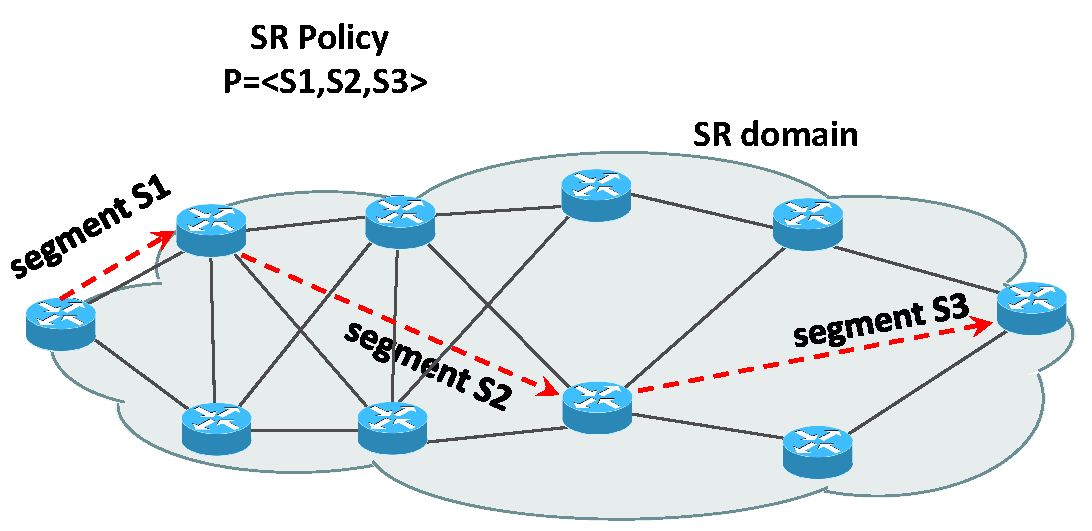
\includegraphics[width=0.45\textwidth]{fig/sr-domain-simple.pdf}
    \caption{SR policy and segments}
    \label{fig:sr_policy_and_segments}
    \vspace{-3ex}
\end{figure}
%pdf generated by powerpoint sr-domain-simple.pptx, printing on PDF creator 
% settings, advanced settings, papersize "postscript custom page setup"
% true type fonts "download as softfonts"
% width 90 mm height 185 mm % print quality 1200 dpi 
% in powerpoint settings "High quality" from the slides print setting
% NB powerpoint 2003 prints better images (300KB) than powerpoint 365 (70KB)


\begin{figure}
    \centering
    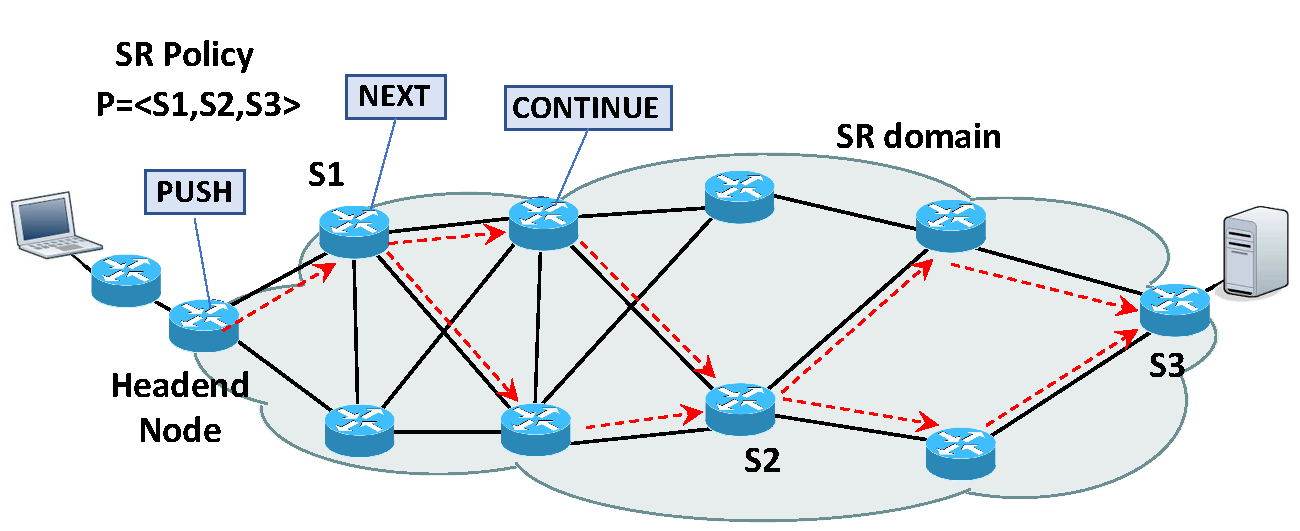
\includegraphics[width=0.45\textwidth]{fig/sr-domain.pdf}
    \caption{Segment Routing operations}
    \label{fig:sr_operations}
    \vspace{-3ex}
\end{figure}
%pdf generated by powerpoint sr-domain.pptx, printing on PDF creator 
% settings, advanced settings, papersize "postscript custom page setup"
% true type fonts "download as softfonts"
% width 90 mm height 220 mm % print quality 1200 dpi 
% in powerpoint settings "High quality" from the slides print setting
% NB powerpoint 2003 prints better images (300KB) than powerpoint 365 (70KB)

The segments can be classified into \textit{Global Segments} and \textit{Local Segments}. Global Segments correspond to instructions that are globally valid in an SR domain. Local segments correspond to instructions that are valid within a single node. The typical example of a global segment is an instruction to forward packets toward a given destination IP network or a destination IP node. Considering that an IGP (Interior Gateway Protocol) routing protocol (e.g. OSPF or ISIS) is used in the SR domain, these instructions are called \textit{IGP-prefix segment} and \textit{IGP-node segment} (or simply prefix segment and node segment). All nodes in the SR domain can execute the prefix segment or node segment instructions by considering the path toward the destination network or destination node in their routing table. The most important example of local segment is the instruction to forward a packet to a node identified as adjacent by the IGP routing protocol. This corresponds to sending the packet on a specific outgoing interface and can be executed only on a specific node. This instruction is called \textit{IGP-Adjacency Segment}. Thanks to the use of IGP-Adjacency segments, it is possible to prove that any path across an SR domain can be expressed by an SR Policy (which can include a combination of global and local segments) \cite{pmsr}. Local segments can also be used to represent service instructions to be executed in a given node. The mapping of global and local segment into Segment Identifiers (SIDs) and the distribution of the SIDs in an SR domain are different for SR-MPLS and SRv6) and will be discussed in the next subsections.

The \textit{IGP-Anycast Segment} is an IGP-Prefix segment that corresponds to an anycast prefix, i.e. a prefix advertised by a set of routers that can be used for High Availability or Load Balancing purposes. 

% OLD VERSION OF THE BINDING SEGMENT EXPLANATION
%The \textit{Binding Segment} is used to associate an SR policy to a SID (called Binding SID or \textit{BSID}). A packet received with the BSID will be steered on the associated SR policy, this means that the packet will be forwarded using the corresponding Segment List. Using the Binding Segment it is possible to separate the processes of packet classification by the enforcing of a specific SR Policy. The SR policy can be changed over time (and can be executed in a different node) with no need to change the classification process. This improves the scalability, resilience and service independence of the solutions based on Segment Routing.

% NEW VERSION OF THE BINDING SEGMENT EXPLANATION
The \textit{Binding Segment} is used to associate an SR policy (i.e. a Segment List) to a SID (called Binding SID or \textit{BSID}) in a given node. This means that the node that processes the Binding SID replaces this segment with a Segment List: a packet received with the BSID as active segment will be steered on the associated SR policy. In this way, the packet classification can be executed by a node X that adds the Binding SID in the SR Header. The node X does not need to know the details of the SR policy to be applied (i.e. the Segment List). Thanks to the BSID the packet will be forwarded to a node Y that is able to apply the Segment List. As an example, the node X can classify traffic for a given destination network N that requires \dq{low latency} and traffic for the same destination network N that requires \dq{low loss}. Node Y is an ingress node of a backbone that provides connectivity toward the network N. Two SR policies (\dq{low latency} and \dq{low loss}) are used to forward traffic toward the network N across the backbone. The respective lists of segments can change over time, based on Traffic Engineering considerations. Upon these changes, the node Y is re-configured to apply the current SR policy to the packets identified by the Binding SID. Node X does not need to be reconfigured, as the Binding SIDs remain constant over time. This approach improves the scalability, resilience and service independence of the solutions based on Segment Routing.

Table~\ref{table-sr-mappings} summarizes the mapping of the SR concepts into the two data planes (MPLS and IPv6) and will be discussed in the next two subsections. \revnew{It is interesting to note how some requirements that led to the definition of the SR solutions are currently fulfilled by \dq{Over the top} (OTT) providers to deliver services with less degree of flexibility using tunneling technologies such as GRE (Generic Routing Encapsulation) \cite{rfc2784} and VXLAN (Virtual eXtensible LAN) \cite{rfc7348}. These technologies allow to encapsulate traffic and forward the packets toward remote nodes according to an overlay logical topology. Unfortunately, they come with a penalty, for example a protocol like VXLAN needs an L3 underlay to transport traffic and loses full L3 forwarding capabilities such as ECMP forwarding \cite{line}. They are not really forms of source routing and do not allow to define way-points where to stick the traffic. To further elaborate, in \cite{line} it is reported an interesting use case where multi-tenancy in a datacenter fabric has been implemented using SRv6 as overlay/underlay instead of the commonly used technologies like VXLAN with a drastic simplification of the architecture. For Service Function Chaining (SFC) scenarios, the Network Service Header (NSH) \cite{rfc8300} is a solution that works on top of tunneling technologies. Therefore NSH can be used in combination with Segment Routing, when SR is only used as tunneling mechanism (enhanced with Traffic Engineering features). On the other hand NSH can be seen as an alternative to Segment Routing for implementing the Service Function Chaining functionality. In this respect, \cite{metaswitch} and \cite{mayer2019efficient} elaborate on Service Function Chaining scenarios where SRv6 would allow to fully replace the NSH layer leading to a simplification of the infrastructure and reducing the load on the devices.}

\begin{table}
\caption{\\Mapping SR concepts into SR-MPLS and SRv6}
\label{table-sr-mappings}
\begin{tabular}{|l|l|l|}
\hline
\textbf{Generic SR}                                          & \textbf{SR-MPLS} & \textbf{SRv6}                                                                                                                               \\ \hline
SR Policy                                                    & Label Stack      & \begin{tabular}[c]{@{}l@{}}Segment List (of IPv6\\ addresses) in the SR Header\end{tabular}                                                 \\ \hline
Active Segment                                               & Topmost Label    & \begin{tabular}[c]{@{}l@{}}IPv6 address indicated\\ in the IPv6 Destination Address\end{tabular}                                                  \\ \hline
\begin{tabular}[c]{@{}l@{}}PUSH\\ Operation\end{tabular}     & Label Push       & \begin{tabular}[c]{@{}l@{}}Adding an IPv6 in the Segment\\ List in the SR Header\end{tabular}                                               \\ \hline
\begin{tabular}[c]{@{}l@{}}NEXT\\ Operation\end{tabular}     & Label POP        & \begin{tabular}[c]{@{}l@{}}Decrementing the Segment Left\\ field, copying the active segment\\ in the IPv6 Destination Address\end{tabular} \\ \hline
\begin{tabular}[c]{@{}l@{}}CONTINUE\\ Operation\end{tabular} & Label Swap       & \begin{tabular}[c]{@{}l@{}}Forwarding according to IPv6\\ Destination Address\end{tabular}                                                  \\ \hline
\end{tabular}
\end{table}

\subsection{MPLS data plane (SR-MPLS)}
\label{sec:mpls-data plane}

The MPLS data plane (SR-MPLS) is specified in \cite{id-segment-routing-mpls}. For SR-MPLS, Segment Routing does not require any change to the MPLS forwarding plane. An SR Policy is instantiated through the MPLS Label Stack: the Segment IDs (SIDs) of a Segment List are inserted as MPLS Labels. 
The classical forwarding functions available for MPLS networks allow implementing the SR operations. The PUSH operation corresponds to the Label Push function, i.e. pushing an MPLS label on a packet. The NEXT operation corresponds to the Label Pop function, i.e. removing the topmost label. The CONTINUE operation corresponds to the Label Swap function, i.e. associating an incoming label with an outgoing interface and outgoing label and forwarding the packet on the outgoing interface. 
The encapsulation of an IP packet into an SR-MPLS packet is performed at the edge of an SR-MPLS domain, reusing the MPLS Forwarding Equivalent Class (FEC) concept. A Forwarding Equivalent Class (FEC) can be associated with an SR Policy.

The mapping of Segments to MPLS Labels (SIDs) is a critical process in the SR-MPLS data plane. In the general case, different routers in the SR domain could have different available ranges of labels to be used for Segment Routing. Therefore each router can advertise its own available label space to be used for Global Segments called \textit{SRGB - Segment Routing Global Block} (in general, this label space can even be composed of a set of non contiguous blocks). For this reason, in the SR domain the Global Segments are identified by an index, which has to be re-mapped into a label taking into account the node that will process the label. Assuming that the SRGB of a node is a label range starting from 10000, for a Global Segment with index X, the node needs to receive the label 10000+X. As an example, in Fig.~\ref{fig:mpls-data plane}~A we consider how to implement the SR policy described in Fig.~\ref{fig:sr_operations} using the SR-MPLS data plane. We assume that different nodes are using different SRGBs. The SRGBs of the nodes and the segment index associated to the segments S1, S2 and S3 are shown in the gray rectangle. The headend node needs to consider in advance which is the SRGB of the nodes that will perform the NEXT operation the segments, because the label for the next segments needs to be crafted accordingly. In particular, the initial label for segment S2 set by the headend node will be 1002, i.e. the SRGB of node S1 (1000) plus the index for segment S2 (2). Node S1 will have to modify the label to 4002 if the packet is forwarded to node N4 (whose SRGB is 4000) or to label 6002 if the packet is forwarded to node N6 (whose SRGB is 6000). Both nodes N4 and N6 will remap (swap) the label to 2002 when forwarding the packets to S2. The initial label for node S3 set by the headend node is 2003, i.e. the SRGB of node S2 (2000) plus the index for segment S3 (3). This label will reach node S2 unmodified, then it will be properly processed by node S2 that will remap (swap) it considering the SRGB of the next hop in the path toward node S3. This remapping process complicates the operations and the troubleshooting. There are also services (e.g. involving anycast segments) that cannot be realized if different SRGBs are used by different nodes. For this reason, \cite{rfc8402} strongly recommends that an identical range of labels (SRGB) is used in all routers, so that a Global Segment will always be mapped to the same SID (MPLS label) in all nodes. In Fig~\ref{fig:mpls-data plane}~B we present the mapping of the same SR policy described in Fig.~\ref{fig:sr_operations} under the suggested operating mode in which an identical SRGB is used in all nodes. We observe that the MPLS labels do not need to be remapped, so that the same label consistently identifies the same global segment throughout the SR domain.

\begin{figure}
    \centering
    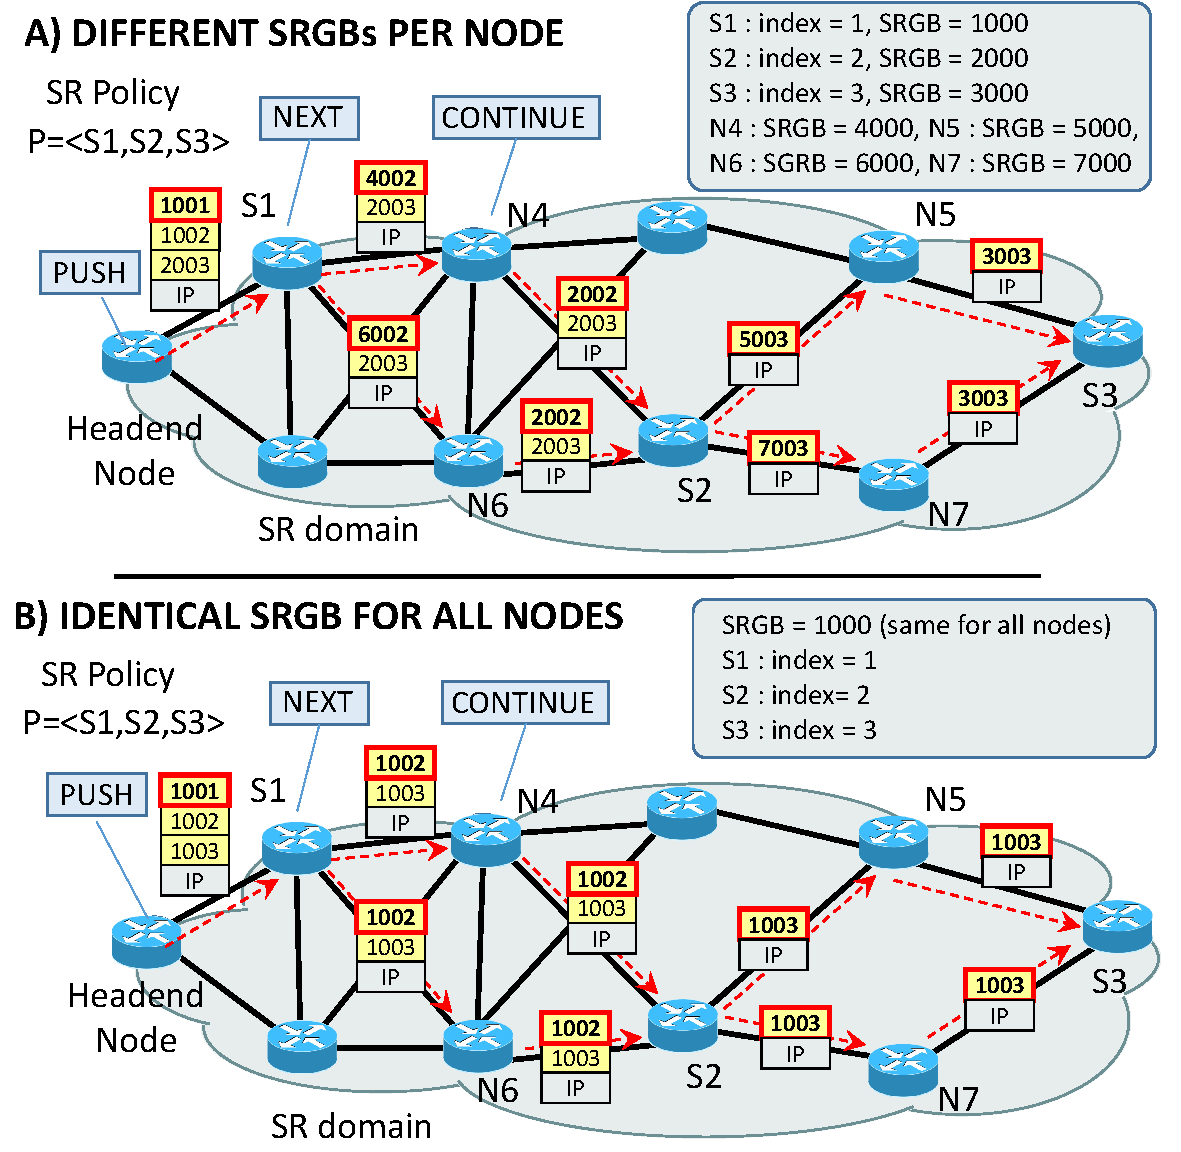
\includegraphics[width=0.48\textwidth]{fig/srgb-mpls-ok.pdf}
    \caption{SR-MPLS data plane: mapping segments to labels using the SRGB}
    \label{fig:mpls-data plane}
    \vspace{-3ex}
\end{figure}
%pdf generated by powerpoint, printing on PDF creator 
% settings, advanced settings, papersize postscript custom page setup
% width 195 mm height 200 mm % print quality 1200 dpi % true type download as softfonts
% in powerpoint settings "High quality" from the slides print setting


\subsection{IPv6 data plane (SRv6)}
\label{sec:ipv6 data plane}

For the IPv6 data plane (SRv6), a new type of IPv6 Routing Extension Header, called Segment Routing Header (SRH) has been defined in \cite{ietf-6man-segment-routing-header}. The format of the SRH is shown in Fig.~\ref{fig:sr-header}. The SRH contains the Segment List (SR Policy) as an ordered list of IPv6 addresses: each address in the list is a SID. A dedicated field, referred to as \textit{Segments Left}, is used to maintain the pointer to the active SID of the Segment List. To explain the SRv6 data plane, we consider three categories of nodes: Source SR nodes, Transit nodes and SR Segment Endpoint nodes. A Source SR node corresponds to the \textit{headend} node discussed above. It can be a host originating an IPv6 packet, or an SR domain ingress router encapsulating a received packet in an outer IPv6 header. In Fig.~\ref{fig:srv6-data plane} we consider the latter case, the Source SR node is an edge router that encapsulates a packet (which can be IPv6, IPv4 or even a Layer 3 frame) into an outer IPv6 packet and inserts the SR Header (SRH) as a Routing Extension Header in the outer IPv6 header. The encapsulated packet is indicated as Payload in Fig.~\ref{fig:srv6-data plane}. The Segment List in the SRH is composed of S1, S2 and S3 which are stored in reverse order (the fist SID is S3, the last segment in the SR policy). The Segment Left field is set to 2, so that the active segment is S1, represented in red in the figure. The Source SR node sets the first SID of the SR Policy (S1) as IPv6 Destination Address of the packet. These operations correspond to a sequence of the PUSH operations described above. The SR Segment Endpoint node receives packets whose IPv6 destination address is locally configured as a segment. The SR Segment Endpoint node inspects the SR header: it detects the new active segment, i.e. the next segment in the Segment List, modifies the IPv6 destination address of the outer IPv6 header and forwards the packet on the basis of the IPv6 forwarding table. These operations correspond to the NEXT operation described above. In Fig.~\ref{fig:srv6-data plane}, we can see that S1 is the first SR Endpoint node, it decrements the Segment Left fields to 1, making S2 the active segment, and sets S2 as IPv6 Destination Address. A Transit node forwards the packet containing the SR header as a normal IPv6 packet, i.e. on the basis of the (outer) IPv6 destination address, because the IPv6 destination address does not locally correspond to a segment. These operations correspond to the CONTINUE operation. In Fig.~\ref{fig:srv6-data plane}, nodes N4, N5, N6 and N7 are Transit nodes, which perform a regular forwarding of the packet toward the IPv6 Destination Address. Note that in SRv6 the Transit nodes do not need to be SRv6 aware, as every IPv6 router can act as an SRv6 Transit node. 

\begin{figure}
    \centering
    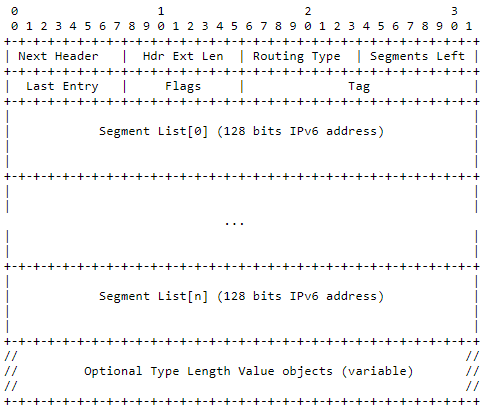
\includegraphics[width=0.8\columnwidth]{fig/sr-header.png}
    \caption{Segment Routing Header}
    \label{fig:sr-header}
%    \vspace{-3ex}
\end{figure}

\begin{figure}
    \centering
    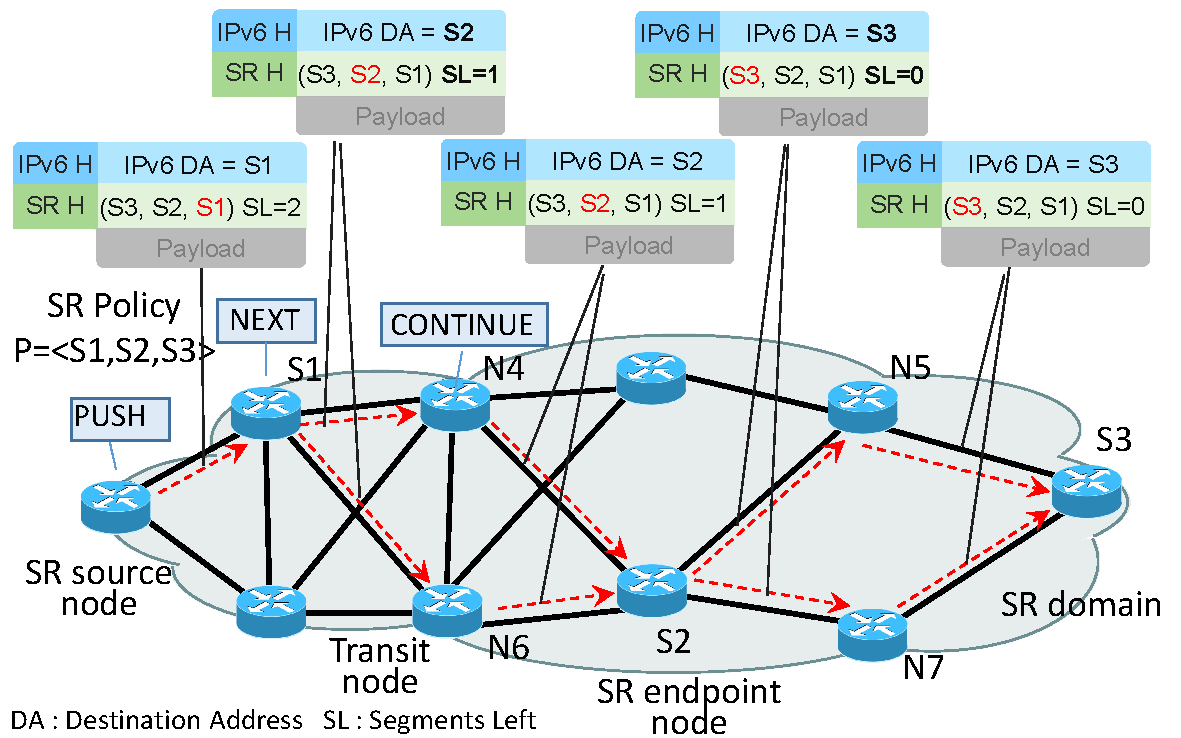
\includegraphics[width=0.48\textwidth]{fig/srv6-example.pdf}
    \caption{SRv6 data plane operations}
    \label{fig:srv6-data plane}
    \vspace{-3ex}
\end{figure}
%pdf generated by powerpoint, printing on PDF creator 
% settings, advanced settings, papersize postscript custom page setup
% width 118 mm height 230 mm % print quality 1200 dpi % true type download as softfonts
% in powerpoint settings "High quality" from the slides print setting

In the given example, the PUSH operation is performed by encapsulating a packet (IPv6, IPv4 or Layer 2 frame) into an outer IPv6 packet with a Segment Routing Header. Another possibility is to perform the \textit{insertion} of an SRH as a new header between the IPv6 header and the Next Header (e.g. the Trasport Layer Header, TCP or UDP), without encapsulating the packet in a new IPv6 packet. This option only applies to IPv6 packets and it is especially suited in case the source host is acting as Source SR node (Headend node). 

In addition to the basic operations (PUSH/ NEXT/ CONTINUE), the \textit{SRv6 Network Programming} model \cite{id-srv6-network-prog} describes a set of functions that can be associated to segments and executed in a given SRv6 node. Examples of such functions are: different types of packet encapsulation (e.g. IPv6 in IPv6, IPv4 in IPv6, Ethernet in IPv6), corresponding decapsulation, lookup operation on a specific routing table (e.g. to support VPNs). The list of functions described in \cite{id-srv6-network-prog} (discussed in section~\ref{sec:sr_net_prog}) is not meant to be exhaustive, as any function can be associated to a segment identifier in a node. Obviously, the definition of a standardized set of segment routing functions facilitates the deployment of SR domains with interoperable equipment from multiple vendors.

According to \cite{id-srv6-network-prog}, we can revisit the notion of Segment IDentifier (SID) taking into account that IPv6 addresses are used as SIDs in SRv6. A 128 bit SID can be logically split in three fields and interpreted as LOCATOR:FUNCTION:ARGS (in short LOC:FUNCT:ARG) where LOC includes the L most significant bits, FUNCT the following F bits and ARG the remaining A bits, where 128=L+F+A. The locator corresponds to an IPv6 prefix (for example with a length of 48, 56 or 64 bits) that can be distributed by the routing protocols and provides the reachability of a node that hosts a number of functions. The length L of the locator is not fixed and can be chosen by each operator for its own SR domain (also independently for different nodes). All the different functions residing in a node can share the same locator and have a different FUNCT code, so that their SIDs will be different. From the routing point of view, the solution is very scalable as a single prefix is distributed for a node that implements a potentially large number of functions, with limited impact on the routing tables of the nodes in the SR domain. The ARG bits can be used to provide information (arguments) to a function. They are optional: if A=0, the SID can be simply decomposed in two fields as LOC:FUNCT, and 128=L+F. \revnew{A SID split into LOC:FUNCT:ARG is a global segment if the LOC prefix is routable in the SRv6 domain, which is the typical case. It is also possible to define local segments in SRv6, i.e. non routable SIDs that can be executed by a node and needs to be preceded a global SID used to forward the packet to the node. Anyway, the use of such local SIDs can be avoided as the FUNCT part of a global SID in the form LOC:FUNCT:ARG can represent the needed local function.}

\subsection{SRv6 Network Programming Model}
\label{sec:sr_net_prog}

The SRv6 Network Programming model is defined in \cite{id-srv6-network-prog}. It consists in combining functions that can reside in different nodes to achieve \textit{a networking objective that goes beyond mere packet routing}. The functions described in \cite{id-srv6-network-prog} can support valuable services and features like layer 3 and layer 2 VPNs, traffic engineering, fast rerouting. The Network Programming model offers the possibility to implement virtually any service by combining the basic functions in a \textit{network program} that is embedded in the packet header. As shown in Fig.~\ref{fig:sr-header}, the SRH can include an optional section that carries Type Length Value (TLV) objects. These TLV objects can be defined to carry information that needs to be elaborated by one or more segments of an SR policy (Segment List). For example, the so-called HMAC TLV can be added and used to verify that an SRH header has been created by an authorized node and that the segment list is not modified in transit. Another potential use of TLV objects is for exchanging Operation and Maintenance (OAM) information among the nodes of the SR domain.

%SRv6 implementations have been revised several times to keep up with the evolution of the SRv6 network programming concepts defined in~\cite{id-srv6-network-prog}.
\revnew{The draft \cite{id-srv6-network-prog} defines two different sets of SRv6 behaviors, known as \textit{SR policy headend} and \textit{endpoint} behaviors. With reference to Fig.~\ref{fig:srv6-data plane}, SR policy headend behaviors are executed in the SR source nodes, while endpoint behaviors in SR endpoint nodes (e.g. S1, S2, S3). \textit{SR policy headend} behaviors steer received packets into the SRv6 policy matching the packet attributes. Each SRv6 policy has a list of SIDs to be attached to the matched packets. Note that in earlier version of \cite{id-srv6-network-prog}, the SR policy headend behaviors were referred to as \textit{transit} behaviors, which was misleading because the same attribute (\textit{transit}) was applied to the SR source nodes and to the transit nodes not doing any operation. On the other hand, an SRv6 \textit{endpoint} behavior, also known as behavior associated with a SID, represents a function to be executed on packets at a specific location in the network. Such function can be a simple routing instruction, but also any advanced network function (e.g., firewall, NAT).}
%If the IPv6 destination address \dq{is neither a local address nor a local SID} then the node forwards the packet without inspecting the SRH. 

\revnew{Table~\ref{tab:sr-behaviors} reports a non-exhaustive list of SRv6 behaviors, listing the documents that provide their description.
%in \cite{id-srv6-network-prog}: \textit{T.Insert}, \textit{T.Encaps}, \textit{T.Encaps.L2}, \textit{End}, \textit{End.X}, \textit{End.T}, \textit{End.DX6}, \textit{End.DX4}, \textit{End.DT6}, \textit{End.DT4}, \textit{End.DT46}, \textit{End.DX2}.
The \textit{H.Encaps} behavior encapsulates an IPv6 packet, which becomesthe inner packet of an IPv6-in-IPv6 packet. The outer IPv6 header carries the SRH header, which includes the SIDs list. The \textit{H.Encaps.L2} behavior is the same as the \textit{H.Encaps} behavior, with the difference that \textit{H.Encaps.L2} encapsulates the full received layer-2 frame rather than the IP packet (Ethernet over IPv6 encapsulation). The \textit{H.Insert} behavior inserts an SRH in the original IPv6 packet, immediately after the IPv6 header and before the transport level header. The original IPv6 header is modified, in particular the IPv6 destination address is replaced with the IPv6 address of the first segment in the segment list, while the original IPv6 destination address is carried in the SRH header as the last SID of the SIDs list.}

\revnew{The \textit{End} behavior represents the most basic SRv6 function among the endpoint behaviors. It replaces the IPv6 destination address of the packet with the next SID in the SIDs list. Then, it forwards the packet by performing a lookup of the updated IPv6 Destination Address in the routing table of the node. We will refer to the lookup in the routing table as \textit{FIB lookup}, where FIB stands for Forwarding Information Base. The \textit{End.T} behavior is a variant of the \textit{End} behavior, %relying on the multiple tables lookup functionality: 
in which the FIB lookup is performed in a specific IPv6 table associated with the SID rather than in the main routing table. The \textit{End.X} behavior is another variant of the \textit{End} behavior, in which the packet is directly forwarded to a specified of the layer-3 adjacency bound to the SID, without performing a FIB lookup of the IPv6 destination address.}

\revnew{The \textit{End.DT6} behavior pops out the SRv6 encapsulation and performs a FIB lookup of the IPv6 destination address of the exposed inner packet in a specific IPv6 table associated with the SID. It is possible to associate the default IPv6 routing table with the SID, in this case the inner IPv6 packets will be decapsulated and then forwarded on the basis of its IPv6 destination address according to the default routing of the node. The \textit{End.DX6} behavior removes the SRv6 encapsulation from the packet and forwards the resulting IPv6 packet to a specific layer-3 adjacency associated to the SID. \textit{End.DT4} and \textit{End.DX4} are respectively the IPv4 variant of \textit{End.DT6} and \textit{End.DX6}, i.e. they are used when the encapsulated packet is an IPv4 packet. The \textit{End.DX2} behavior is used for packets encapsulated at Layer 2 (e.g. with H.Encaps.L2). It pops out the SRv6 encapsulation and forwards the resulting L2 frame via an output interface associated to the SID.} 

\begin{table}[htbp]
\caption{(Non-exhaustive) list of SRv6 behaviors}
\label{tab:sr-behaviors}
\centering
\begin{tabular}{|l|c|}
\hline
Behavior          &  Defined in \\
\hline
H.Encaps          & srv6-network-programming \cite{id-srv6-network-prog} \\
\hline
%H.Encaps.Red      & srv6-network-programming \cite{id-srv6-network-prog} \\
%\hline
H.Insert          & srv6-network-programming \cite{id-srv6-network-prog}  \\
\hline
%H.Insert.Red      & srv6-network-programming \cite{id-srv6-network-prog} \\
%\hline
H.Encaps.L2       & srv6-network-programming \cite{id-srv6-network-prog} \\
\hline
%H.Encaps.L2.Red   & srv6-network-programming \cite{id-srv6-network-prog} \\
%\hline
End               & srv6-network-programming \cite{id-srv6-network-prog} \\
\hline
End.T             & srv6-network-programming \cite{id-srv6-network-prog} \\
\hline
End.X             & srv6-network-programming \cite{id-srv6-network-prog} \\
\hline
End.DT4           & srv6-network-programming \cite{id-srv6-network-prog} \\
\hline
End.DT6           & srv6-network-programming \cite{id-srv6-network-prog} \\
\hline
%End.DT46          & srv6-network-programming \cite{id-srv6-network-prog} \\
%\hline
End.DX4           & srv6-network-programming \cite{id-srv6-network-prog} \\
\hline
End.DX6           & srv6-network-programming \cite{id-srv6-network-prog} \\
\hline 
End.DX2           & srv6-network-programming \cite{id-srv6-network-prog} \\
\hline
%End.DX2V          & srv6-network-programming \cite{id-srv6-network-prog} \\
%\hline
%End.DT2U          & srv6-network-programming \cite{id-srv6-network-prog} \\
%\hline
%End.DT2M          & srv6-network-programming \cite{id-srv6-network-prog} \\
%\hline
%End.B6.Insert     & srv6-network-programming \cite{id-srv6-network-prog} \\
%\hline
%End.B6.Insert.Red & srv6-network-programming \cite{id-srv6-network-prog} \\
%\hline
%End.B6.Encaps     & srv6-network-programming \cite{id-srv6-network-prog} \\
%\hline
%End.B6.Encaps.Red & srv6-network-programming \cite{id-srv6-network-prog} \\
%\hline
%End.BM            & srv6-network-programming \cite{id-srv6-network-prog} \\
%\hline
\hline
End.AS            & service-programming (SFC) \cite{id-sr-service-programming} \\
\hline
End.AD            & service-programming (SFC) \cite{id-sr-service-programming} \\
\hline
End.AM            & service-programming (SFC) \cite{id-sr-service-programming} \\
\hline
\hline
T.M.Tmap          & mobile-uplane \cite{id-srv6-mobile-uplane} \\
\hline
End.M.GTP4.E      & mobile-uplane \cite{id-srv6-mobile-uplane} \\
\hline
End.M.GTP6.D      & mobile-uplane \cite{id-srv6-mobile-uplane} \\
\hline
End.M.GTP6.E      & mobile-uplane \cite{id-srv6-mobile-uplane} \\
\hline
\end{tabular}
\end{table}

% fast path vs slow path?

% My SID table ?

\subsection{Control plane for SR and relation with SDN}
\label{sec:sr_control_plane}

Control Plane operations are needed to complement the data plane functionality and provide a complete solution for Segment Routing. The Control Plane can be based on a fully distributed approach, in which the routers are capable to take independent decisions to setup and enforce the SR Policies, it can rely on a centralized SR controller that takes decision and instructs the routers following the SDN principles, or on a combination of the two approaches (hybrid solution). 

For the SR-MPLS data plane, the definition of a fully distributed approach has been worked out within the IETF, with the definition of extensions to the IGP routing protocols (OSPF, ISIS, see \cite{ietf-ospf-segment-routing-extensions} \cite{ietf-ospf-ospfv3-segment-routing-extensions} \cite{ietf-isis-segment-routing-extensions}). 
These extensions to the routing protocols are used by each routers to advertise the different types of IGP-segments (prefix, node, adjacency, anycast) and to distribute some SR configuration information. All other routers in the SR domain will receive this information by means of the IGP routing protocol. This information is needed to map the segments included in an SR policy into SIDs represented as MPLS labels in the SR-MPLS data plane. As we have discussed in subsection \ref{sec:mpls-data plane}, in the general case each router could allocate different ranges of labels to be used for Global Segments. The range of labels used for the global segments by a router, called \textit{SRGB - Segment Routing Global Block} is among the SR configuration information advertised using the routing protocol. We recall that it is strongly recommended to use an identical range of labels (SRGB) in all routers. 

For the IPv6 data plane, the process of advertising the IGP-prefix, IGP-node and IGP-anycast segments is simplified thanks to the use of IPv6 addresses as SIDs. In particular, there is no need to extend the IGP routing protocols to distribute these segment types, represented as IPv6 prefixes that are natively distributed by the routing protocols. Also the definition of a Segment Routing Global Block as in the SR-MPLS is not needed and the operations related to Global Segments can rely on IPv6 addresses that are globally routable in the SR domain. This means that the Control Plane for SRv6 can use the regular IGP routing protocols (OSPF, ISIS) to support the basic operations, while extensions are still needed (\cite{id-isis-srv6-extensions} \cite{li-ospf-ospfv3-srv6-extensions}) to distribute IGP-Adjacency segments and other SR configuration information. 

The definition of the control plane for Segment Routing has started from the SR-MPLS data plane and then the SRv6 data plane has inherited most of the functionality, which has been adapted to the new data plane. We observe that an original design goal of the control plane for Segment Routing has been to support the fully distributed approach, in which routers are capable to take autonomous decisions. This allows offering the the same functionality of a traditional MPLS network, which does not need a centralized SDN controller for its operations. On the other hand, we observe now a trend to focus on an hybrid approach, in which distributed routing protocols coexist with an SR controller. This hybrid approach is aligned with the vision of Software Defined Networking that aims at removing complexity from distributed nodes and to centralize control plane function in SDN controllers. In this light, the Segment Routing architecture can be deployed by seeking the right balance between distributed and centralized control. The distributed control is used by the routers to exchange reachability information and evaluate the shortest paths in a traditional way, with no need to interact with the centralized controller. We observe that this is the best approach to provide connectivity in Wide Area Networks in which the control connections between the nodes and the SDN controllers are affected by non-negligible latency and failure probability. Segment Routing can be used for Fast Reroute, by pre-configuring SR policies that provide alternate paths in case of link or node failures and are automatically activated by the node when the failure happens. The pre-calculation of such SR policies can be performed in a distributed mode or can be centralized in a controller. Basic topology information and additional information for Traffic Engineering need be conveyed to the controller, as well as service related information that is advertised by nodes using distributed routing protocols. The SDN controller can receive this information in different ways. For example, it can participate to the IGP routing protocol, it can interact with routers in a proprietary way to extract their IGP databases, it can receive information by routers using extensions to BGP-LS (BGP-Link State). Whatever mechanism has been used to retrieve the needed information from the nodes, the SDN controller is in charge to take decisions about the SR policies that implement advanced features or services like Traffic Engineering, VPNs or Service Function Chaining. This approach allows to clearly decouple the data plane operations from the service logic operating in the control plane. The mechanisms and protocols for the SDN controller to enforce the SR policies by configuring the the nodes are left open in the SR architectural definition. As mentioned in \cite{rfc8402}, some options are Network Configuration Protocol (NETCONF), Path Computation Element Communication Protocol (PCEP) \cite{ietf-pce-segment-routing}, and BGP. The Openflow protocol can be used as a mechanism to configure the SR policies only for SR-MPLS, while SRv6 is not supported by the latest standard version of Openflow. An Open Source implementation of a SouthBound API for SRv6 based on gRPC is reported in \cite{ventre2018sdn}. The main characteristic of the Segment Routing solution compared to other SDN solutions is that only the edge nodes needs to be configured to enforce a given SR policy, while the internal nodes do not need to keep state per SR policy. This feature gives a substantial improvement in terms of scalability. 

\subsection{Segment Routing motivations and use cases}

As anticipated in the introduction section, the RFC 5439 \cite{rfc5439} has identified some scalability issues of traditional MPLS networks with Traffic Engineering support. These issues originated the interest in defining a more scalable solution like Segment Routing back in the late `00s. Several use cases and requirements for Segment Routing has been collected in a number of documents. In \cite{rfc7855}, the main use cases identified are: MPLS tunneling (i.e. to support VPN services), Fast ReRoute (FRR), Traffic Engineering (further classified in a number of more specific use cases). A set of Resiliency use cases is described in \cite{rfc8355}. In \cite{rfc8354}, the Segment Routing use cases for IPv6 networks are considered, with a set of exemplary deployment environments for SRv6: Small Office, Access Network, Data Center, Content Delivery Networks, Core Networks.

\begin{comment}
\begin{itemize}
      \item \cite{interconnecting} discusses the capability of SR-MPLS to interconnect a large number of end points with a limited SID space. 
\end{itemize}
\end{comment}



